\chapter*{Preface}  
\addcontentsline{toc}{chapter}{Preface}

\textsc{Note: keep in mind you are reading a \emph{draft} of this tutorial that is being
modified as the students use it (currently in Autumn, 2006).  Although I
apologize for any unforeseen confusion, this is not intended to be a finished
product yet.\textendash TDM}


This document has three primary goals:
\begin{enumerate}
\item It should introduce students to the minimal amount of graphical programming required
  to competently program embedded controllers.  Although this is presented in
  terms of LabVIEW syntax (partially because this effort is being supported by a
  combination of the National Instruments Foundation and the National Science
  Foundation), the basic structure of how graphical programming can be used to
  allow students to do the majority of programming themselves is not dependent
  on LabVIEW.  Other graphical programming languages (such as MATLAB/Simulink)
  can be employed in a nearly identical manner.
\item It should provide control systems laboratories that are open-ended enough
  to take advantage of the fact that students can write their own code.  Among
  other things, this means that students are in charge of nearly all the
  implementation.
\item It should lastly provide a series of laboratories that complement a more
  modern approach to understanding control theory.  In particular, the reader
  should note that there are almost no formulae presented here\textendash instead the
  students are generally required to derive the relevant transformations and
  control laws themselves.  (This is possible because they are not spending all
  their time programming in a more traditional language such as C/C++.)
\end{enumerate}
The direction taken in this tutorial/laboratories is by no means unique and
merely reflects the belief of the author that traditional laboratories have been
too limited in what the students can try.  We have had substantial success with
the open-ended structure of the labs presented here, as documented in
\cite{murphey-ace2006}.

The reader should note that just like LabVIEW is not intrinsically a part of
this laboratory structure, neither is the Educational Control Products (ECP)
Torsional Disk System.  We are currently in the process of extending the basic
structure of these labs to other experimental devices.  


Lastly, the author would like to thank National Instruments and the National
Instruments Foundation for their support of the laboratory.  Moreover, the
author would like to thank the National Science Foundation for supporting the
ongoing assessment of this laboratory.


\noindent Todd Murphey

%\begin{figure}[h!]
%\centering
%\includegraphics[width=6in]{template/graphic}
%\caption{A LabVIEW-related graphic}
%\label{fig-LabVIEWgraphic}
%\end{figure}

%\begin{wrapfigure}[15]{r}{2in}
%\begin{center}
%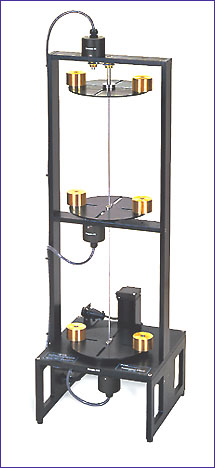
\includegraphics[height=4in]{Lab2/model205}
%\end{center}
%\caption{The ECP Torsional Disk System.}
%\label{fig-ecp}
%\end{wrapfigure}


%% Local Variables:
%% TeX-master: "../LVmanual.tex"
%% End:

